\section{开关?电阻?(40pts)}
Nahida发现了一个古老的须弥电路图,如图\ref{switch} 所示,她想一会后意识到这个具有把开关当成电阻的功能。请你也来学习一下她的芝士吧!
\begin{figure}[htbp]
	\centering
	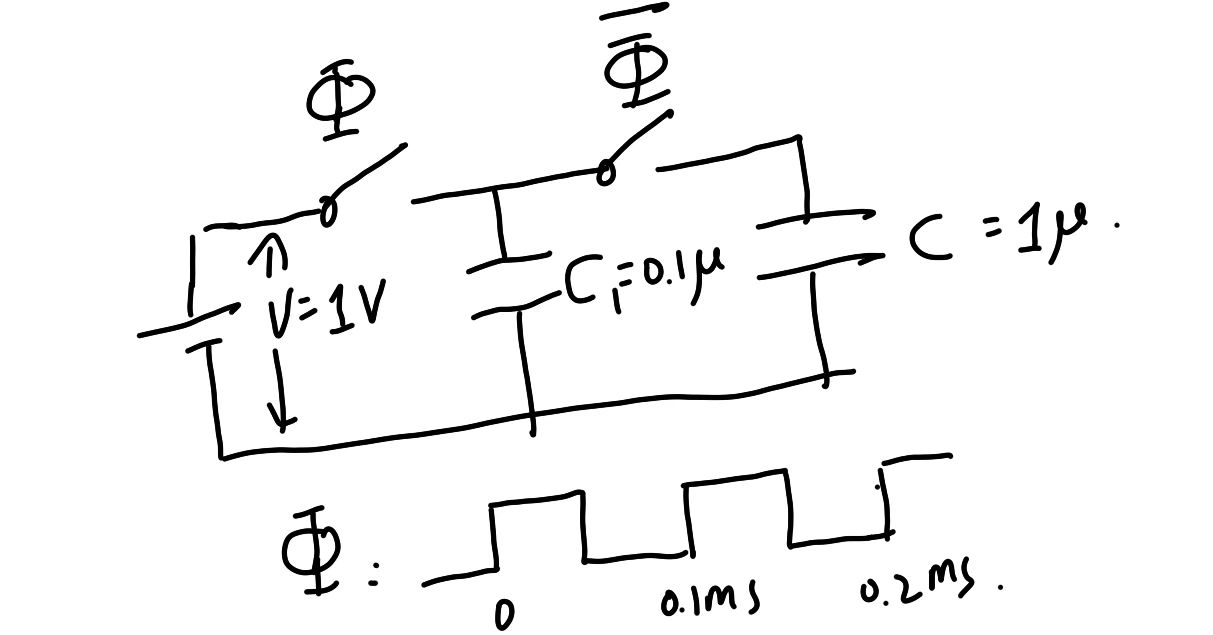
\includegraphics[width=0.5\textwidth]{switch}
	\caption{这是一个简单的电路图.}
	\label{switch}
\end{figure}
\begin{figure}[htbp]
	\centering
	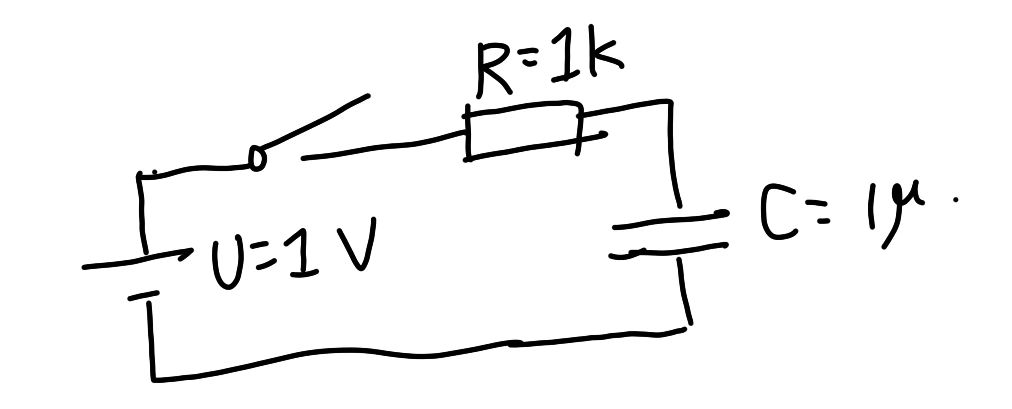
\includegraphics[width=0.5\textwidth]{RC}
	\caption{这真的是一个简单的电路图.}
	\label{RC}
\end{figure}
\begin{enumerate}
	\item 请求出图\ref{RC} 中的电容电压随时间的变化关系式\(V_c(t)\) (4pts)
	\item 请求出图\ref{switch} 中的电容电压随时间的变化关系式\(V_c'(t)\)。图示中有两个开关(cmos管)受到信号\(\Phi\)的控制,两个开关的信号恰好相反,只有当高电平的时候开关才会闭合。 硬件参数已经如图所示(24pts)
	\item 请给出若要把图示的开关完全等效为一个电阻\(R\)的条件。(12pts)
\end{enumerate}